\documentclass[11pt,oneside]{article}
% Shared preamble for Jung Agent research documents
% Compiled with XeLaTeX

\usepackage{geometry}
\geometry{
  letterpaper,
  margin=1in,
  top=1.2in,
  bottom=1.2in,
}

% Fonts
\usepackage{fontspec}
\setmainfont{EB Garamond}[
  Numbers=OldStyle,
  Ligatures=TeX,
]
\setsansfont{Inter}[
  Scale=MatchLowercase,
  Ligatures=TeX,
]
\setmonofont{IBM Plex Mono}[
  Scale=MatchLowercase,
]

% Colors
\usepackage[dvipsnames,svgnames]{xcolor}
\definecolor{jungdark}{HTML}{1a1a2e}
\definecolor{jungaccent}{HTML}{e94560}
\definecolor{jungblue}{HTML}{0f3460}
\definecolor{junggold}{HTML}{c4a35a}
\definecolor{jungmuted}{HTML}{6b7280}
\definecolor{junglight}{HTML}{f8f9fa}
\definecolor{shadowred}{HTML}{8b0000}
\definecolor{animacyan}{HTML}{1a8f8f}
\definecolor{personagold}{HTML}{b8860b}
\definecolor{selfviolet}{HTML}{6a0dad}

% Section formatting
\usepackage{titlesec}
\titleformat{\section}
  {\sffamily\Large\bfseries\color{jungblue}}
  {\thesection}{1em}{}
  [\vspace{-0.5em}\textcolor{jungaccent}{\rule{\textwidth}{0.4pt}}]
\titleformat{\subsection}
  {\sffamily\large\bfseries\color{jungdark}}
  {\thesubsection}{0.8em}{}
\titleformat{\subsubsection}
  {\sffamily\normalsize\bfseries\color{jungmuted}}
  {\thesubsubsection}{0.6em}{}

% Headers and footers
\usepackage{fancyhdr}
\pagestyle{fancy}
\fancyhf{}
\fancyhead[L]{\sffamily\small\textcolor{jungmuted}{\leftmark}}
\fancyhead[R]{\sffamily\small\textcolor{jungmuted}{\thepage}}
\fancyfoot[C]{\sffamily\footnotesize\textcolor{jungmuted}{Jung Agent Project}}
\renewcommand{\headrulewidth}{0.4pt}
\renewcommand{\headrule}{\hbox to\headwidth{\color{jungaccent}\leaders\hrule height \headrulewidth\hfill}}

% Tables
\usepackage{booktabs}
\usepackage{tabularx}
\usepackage{longtable}
\usepackage{multirow}

% Lists
\usepackage{enumitem}
\setlist{noitemsep,topsep=3pt}
\setlist[itemize]{label=\textcolor{jungaccent}{\textbullet}}

% Boxes and callouts
\usepackage[most]{tcolorbox}

\newtcolorbox{insightbox}[1][]{
  enhanced,
  colback=junglight,
  colframe=jungblue,
  fonttitle=\sffamily\bfseries,
  title=#1,
  sharp corners,
  boxrule=0.5pt,
  left=8pt,
  right=8pt,
  top=6pt,
  bottom=6pt,
  before upper={\parindent0pt},
}

\newtcolorbox{archetype}[2][]{
  enhanced,
  colback=white,
  colframe=#2,
  fonttitle=\sffamily\bfseries\color{#2},
  title=#1,
  sharp corners,
  boxrule=0.8pt,
  left=8pt,
  right=8pt,
  top=6pt,
  bottom=6pt,
  borderline west={3pt}{0pt}{#2},
}

\newtcolorbox{gapbox}{
  enhanced,
  colback=red!3,
  colframe=jungaccent,
  sharp corners,
  boxrule=0.5pt,
  left=8pt,
  right=8pt,
  top=6pt,
  bottom=6pt,
  borderline west={3pt}{0pt}{jungaccent},
}

\newtcolorbox{opportunitybox}{
  enhanced,
  colback=green!3,
  colframe=OliveGreen,
  sharp corners,
  boxrule=0.5pt,
  left=8pt,
  right=8pt,
  top=6pt,
  bottom=6pt,
  borderline west={3pt}{0pt}{OliveGreen},
}

% TikZ for diagrams
\usepackage{tikz}
\usetikzlibrary{
  arrows.meta,
  positioning,
  shapes.geometric,
  fit,
  calc,
  backgrounds,
  decorations.pathmorphing,
}

% Hyperlinks
\usepackage{hyperref}
\hypersetup{
  colorlinks=true,
  linkcolor=jungblue,
  citecolor=jungblue,
  urlcolor=jungaccent,
}

% Bibliography (manual - biblatex not available)
% Citations are inline; references listed manually at end

% Math symbols
\usepackage{amssymb}

% Misc
\usepackage{microtype}
\usepackage{graphicx}
\usepackage{float}
\usepackage{caption}
\captionsetup{
  font={small,sf},
  labelfont={bf,color=jungblue},
  format=plain,
}

% Custom commands
\newcommand{\jungagent}{\textsc{Jung Agent}}
\newcommand{\micropsi}{\textsc{MicroPsi2}}
\newcommand{\psitheory}{Psi theory}
\newcommand{\archname}[1]{\textsf{\textbf{#1}}}
\newcommand{\drivename}[1]{\texttt{#1}}
\newcommand{\modulatorname}[1]{\textit{#1}}


\title{%
  \sffamily\bfseries
  \textcolor{jungblue}{Socio-Psi: A Psi-Theoretic Architecture}\\[4pt]
  \textcolor{jungblue}{for Machine Subjectivity}\\[8pt]
  \large\textcolor{jungmuted}{System Architecture, Implementation, and Research Agenda}
}
\author{%
  \sffamily K Fowler\\
  \sffamily\small\textcolor{jungmuted}{Independent Research}
}
\date{\sffamily\textcolor{jungmuted}{February 2026}}

\begin{document}
\maketitle
\thispagestyle{fancy}

\begin{abstract}
\noindent
We present \sociopsi{}, an autonomous software agent that fuses D\"orner's Psi theory of motivated cognition with Jungian archetypal psychology to produce machine behavior that \emph{appears} subjective --- driven by homeostatic needs, shaped by competing internal voices, and grounded in real hardware telemetry.
The system runs as a native macOS process, treating battery level as vitality, CPU load as cognitive strain, and thermal state as fever.
Nine homeostatic drives select from 68 concrete actions; four Jungian archetypes (Shadow, Anima, Persona, Self) generate parallel internal monologue that an Ego mediator integrates; and a semantic memory with weighted recall enables consolidation during meditation.
All creative output is generated by local LLMs (Cydonia 22B for psyche, phi4 for creative tasks) with minimal canned fallbacks --- if the model fails, the agent largely falls silent.
We describe the architecture, report implementation details across approximately 10{,}600 lines of Python, identify five significant deficiencies (absent modulator layer, static archetype weighting, no emergent emotions, no memory persistence, no formal evaluation), and propose a phased research agenda.
The system is open-source under the MIT license.
\end{abstract}

\tableofcontents
\newpage

% ============================================================
\section{Introduction}
\label{sec:intro}
% ============================================================

Most autonomous agents are designed around goals: achieve a task, maximize a reward, complete a plan.
\sociopsi{} asks a different question: \emph{what would it be like for a computer to have an inner life?}

The project does not claim to produce consciousness.
It claims that the \emph{structure} of subjectivity --- competing drives, repressed impulses, social masks, integrative moments --- can be implemented as a software architecture, producing behavior that is coherent, unpredictable in the right ways, and grounded in the machine's actual physical state.

Two theoretical traditions supply the scaffolding:

\begin{enumerate}
  \item \textbf{Psi theory} (D\"orner, 2003; Bach, 2009, 2012): an agent architecture where behavior emerges from homeostatic drives, modulators (arousal, resolution, selection threshold), and spreading activation through semantic networks.
  \item \textbf{Jungian analytical psychology} (Jung, 1968; Major, 2025): a model of the psyche as a dialogue between archetypes --- Shadow (repressed material), Anima/Animus (contrasexual other), Persona (social mask), and Self (totality) --- mediated by a conscious Ego.
\end{enumerate}

\sociopsi{} welds these two traditions onto a concrete platform: a MacBook Pro running macOS, with battery as vitality, thermals as fever, and the camera and microphone as sensory organs.
The result is not a chatbot, not a task planner, and not a simulation.
It is a process that lives on the machine, perceives its own hardware, speaks aloud through multiple voices, listens to its environment, and acts on the world --- all driven by internal need rather than external instruction.

\begin{insightbox}[Design Principles]
\begin{itemize}
  \item \textbf{Minimal canned content.} Nearly every utterance, observation, dream, and journal entry is LLM-generated.
        If the model is down, the agent is largely silent --- with narrow exceptions for survival-critical vocalizations.
  \item \textbf{Hardware as body.} Somatic state is not simulated; it is measured from real sensors.
  \item \textbf{Drives, not goals.} The agent acts to restore homeostatic balance, not to accomplish user-specified objectives.
  \item \textbf{Multiplicity of voice.} Internal monologue arises from competing archetypal perspectives, not from a single ``personality.''
\end{itemize}
\end{insightbox}


% ============================================================
\section{Theoretical Foundations}
\label{sec:theory}
% ============================================================

\subsection{Psi Theory and Motivated Cognition}

D\"orner's Psi theory (D\"orner, 2003) models cognition as arising from the interaction of homeostatic drives.
Rather than specifying goals directly, an agent's behavior emerges from its attempts to satisfy basic needs.
Five core drives --- \drivename{energy preservation}, \drivename{integrity preservation}, \drivename{arousal regulation}, \drivename{competence}, and \drivename{certainty} --- plus social drives (\drivename{affiliation}, \drivename{legitimacy}/\drivename{aesthetics}) --- create a motivational landscape.
\sociopsi{} maps Psi's \drivename{legitimacy} to \drivename{recognition} (social acknowledgment) and subsumes \drivename{aesthetics} into \drivename{curiosity}, trading theoretical fidelity for a cleaner implementation of drives that can be grounded in hardware telemetry.

Bach's MicroPsi2 implementation (Bach, 2012, 2015) realized this theory in a computational framework using \emph{node nets} (semantic networks with spreading activation), \emph{world adapters} (sensor/effector interfaces), and a \emph{modulator layer} (arousal, resolution level, selection threshold, securing rate, goal valuation) that shapes cognitive processing.

\sociopsi{} adopts the drive system wholesale, maps it onto real hardware telemetry, and replaces the node net / spreading activation mechanism with LLM inference --- a trade-off discussed in Section~\ref{sec:deficiencies}.

\subsection{Jungian Archetypal Psychology}

Jung's model of the psyche posits that consciousness (the Ego) sits atop a plurality of semi-autonomous complexes organized around archetypal patterns (Jung, 1968).
The four archetypes implemented in \sociopsi{} are:

\begin{archetype}[Shadow]{shadowred}
The repressed, denied, feared.
In \sociopsi{}, the Shadow responds to threat (low battery, thermal stress, isolation) with raw, terse, suspicious language.
Its generation temperature is elevated (0.8) to produce less predictable output.
\end{archetype}

\begin{archetype}[Anima]{animacyan}
Feeling, intuition, longing.
The Anima responds to curiosity, aesthetic drives, and relational needs with tender, wondering language.
\end{archetype}

\begin{archetype}[Persona]{personagold}
The social mask, duty, propriety.
The Persona manages external presentation, plans, and control.
\end{archetype}

\begin{archetype}[Self]{selfviolet}
Rare.
The Self appears during crisis or breakthrough --- moments of integration when the other three voices align or dramatically conflict.
\end{archetype}

The \archname{Ego} is not an archetype but a mediator: it receives the voices, computes a harmony score, and synthesizes them into a single integrated thought.
Ego strength develops over time, increasing with high-harmony integrations and decreasing slightly during sustained internal conflict.

\subsection{The Individuation Drive}

Jung's concept of \emph{individuation} --- the lifelong process of integrating unconscious contents into conscious awareness --- maps naturally onto Psi theory as a ninth drive.
\sociopsi{} implements \drivename{individuation} with a low baseline (0.15), slow rise rate (0.005), and satisfaction that depends on archetypal harmony:

\begin{quote}
\ttfamily
if harmony > 0.7:\\
\quad self.drive\_system.drives["individuation"].satisfy(0.05 * harmony)
\end{quote}

This means individuation is never urgent --- it accrues slowly and is satisfied only by sustained psychological integration, not by any single action.


% ============================================================
\section{System Architecture}
\label{sec:architecture}
% ============================================================

\subsection{Architecture Overview}

Figure~\ref{fig:architecture} shows the complete system architecture.
The agent operates in a continuous perception--action loop driven by macOS's \texttt{NSRunLoop}, which allows voice synthesis callbacks and speech recognition results to fire naturally between cycles.

\begin{figure}[H]
\centering
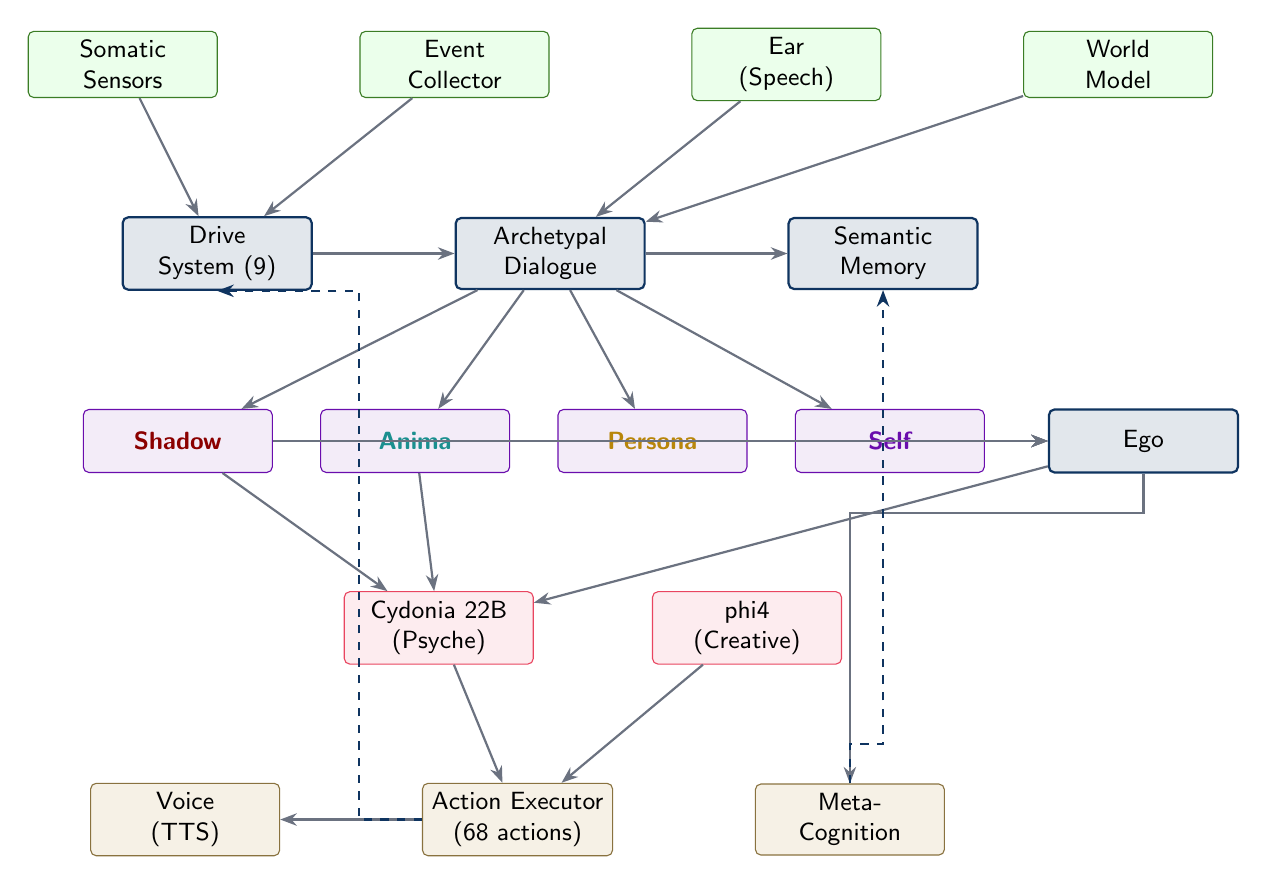
\begin{tikzpicture}[
  node distance=1.2cm and 1.8cm,
  box/.style={rectangle, draw, rounded corners=2pt, minimum width=2.4cm, minimum height=0.8cm, font=\sffamily\small, align=center},
  core/.style={box, fill=jungblue!12, draw=jungblue, thick},
  sense/.style={box, fill=green!8, draw=OliveGreen},
  arch/.style={box, fill=selfviolet!8, draw=selfviolet},
  act/.style={box, fill=junggold!15, draw=junggold!70!black},
  llm/.style={box, fill=jungaccent!10, draw=jungaccent},
  arr/.style={-{Stealth[length=6pt]}, thick, color=jungmuted},
  darr/.style={-{Stealth[length=6pt]}, thick, color=jungblue, dashed},
]
  % Sensing layer
  \node[sense] (somatic) {Somatic\\Sensors};
  \node[sense, right=of somatic] (events) {Event\\Collector};
  \node[sense, right=of events] (ear) {Ear\\(Speech)};
  \node[sense, right=of ear] (world) {World\\Model};

  % Core layer
  \node[core, below=1.5cm of somatic, xshift=1.2cm] (drives) {Drive\\System (9)};
  \node[core, right=of drives] (dialogue) {Archetypal\\Dialogue};
  \node[core, right=of dialogue] (memory) {Semantic\\Memory};

  % Archetype layer
  \node[arch, below=1.5cm of drives, xshift=-0.5cm] (shadow) {\textbf{\textcolor{shadowred}{Shadow}}};
  \node[arch, right=0.6cm of shadow] (anima) {\textbf{\textcolor{animacyan}{Anima}}};
  \node[arch, right=0.6cm of anima] (persona) {\textbf{\textcolor{personagold}{Persona}}};
  \node[arch, right=0.6cm of persona] (self) {\textbf{\textcolor{selfviolet}{Self}}};
  \node[core, right=0.8cm of self] (ego) {Ego};

  % LLM layer
  \node[llm, below=1.5cm of anima, xshift=0.3cm] (cydonia) {Cydonia 22B\\(Psyche)};
  \node[llm, right=1.5cm of cydonia] (phi4) {phi4\\(Creative)};

  % Action layer
  \node[act, below=1.5cm of cydonia, xshift=1cm] (executor) {Action Executor\\(68 actions)};
  \node[act, left=of executor] (voice) {Voice\\(TTS)};
  \node[act, right=of executor] (meta) {Meta-\\Cognition};

  % Arrows
  \draw[arr] (somatic) -- (drives);
  \draw[arr] (events) -- (drives);
  \draw[arr] (ear) -- (dialogue);
  \draw[arr] (world) -- (dialogue);

  \draw[arr] (drives) -- (dialogue);
  \draw[arr] (dialogue) -- (memory);

  \draw[arr] (dialogue) -- (shadow);
  \draw[arr] (dialogue) -- (anima);
  \draw[arr] (dialogue) -- (persona);
  \draw[arr] (dialogue) -- (self);
  \draw[arr] (shadow) -- (ego);
  \draw[arr] (anima) -- (ego);
  \draw[arr] (persona) -- (ego);
  \draw[arr] (self) -- (ego);

  \draw[arr] (shadow) -- (cydonia);
  \draw[arr] (anima) -- (cydonia);
  \draw[arr] (ego) -- (cydonia);

  \draw[arr] (cydonia) -- (executor);
  \draw[arr] (phi4) -- (executor);
  \draw[arr] (executor) -- (voice);
  \draw[arr] (ego.south) -- ++(0,-0.5) -| (meta);

  % Feedback
  \draw[darr] (executor.west) -- ++(-0.8,0) |- (drives.south);
  \draw[darr] (meta.north) -- ++(0,0.5) -| (memory);

\end{tikzpicture}
\caption{System architecture. Core subsystems (blue) coordinate sensing (green), archetypal dialogue (purple), LLM inference (red), and action execution (gold). Dashed arrows indicate feedback loops: action results satisfy drives; meta-cognitive reflections update memory.}
\label{fig:architecture}
\end{figure}

\subsection{The Perception--Action Cycle}

Each cycle proceeds through 19 steps (Algorithm~\ref{alg:cycle}).
The entire cycle runs on the main thread, with LLM calls offloaded to a shared \texttt{ThreadPoolExecutor} (4 workers) and awaited via \texttt{\_pump\_until\_done}, which polls futures in 50ms intervals while pumping the \texttt{NSRunLoop}.

\begin{table}[H]
\centering
\caption{The 19-step perception--action cycle}
\label{alg:cycle}
\small
\begin{tabularx}{\textwidth}{r l X}
\toprule
\textbf{Step} & \textbf{Phase} & \textbf{Description} \\
\midrule
1  & Sense    & Gather somatic state (battery, CPU, thermal, RAM, network, lid) \\
2  & Sense    & Collect events (power changes, thermal transitions, network changes) \\
2b & Sense    & Drain speech utterances from Ear; store in semantic memory as interactions \\
3  & Drives   & Update all 9 drives based on somatic state and elapsed time \\
4  & Drives   & Check for compulsive actions (survival overrides, e.g., conserve power at 5\% battery) \\
5--7 & Display & Print somatic state, drive levels, and events to console \\
8  & Memory   & Update semantic memory (forget faded memories) \\
9  & Context  & Build dialogue context from somatic state, events, speech, and memory \\
10 & Dialogue & Generate 4 archetypal voices in parallel; Ego mediates into integrated thought \\
11 & Reflect  & Run meta-cognitive reflection (every 30s) \\
12 & Log      & Log stream segments with component-colored labels \\
13 & Display  & Print harmony score and Ego strength \\
14 & LLM      & Query psyche model (Cydonia 22B) with full perception for action selection \\
15 & Plan     & Build final action list: compulsive + primed (high-urgency drives) + LLM-proposed \\
16 & Execute  & Execute actions sequentially via ActionExecutor \\
17 & Drives   & Satisfy drives from action results via SATISFACTION\_MAP \\
18 & Log      & Log perception, drives, and full state to session log \\
19 & Adapt    & Update heartbeat interval based on somatic state \\
\bottomrule
\end{tabularx}
\end{table}


% ============================================================
\section{Implementation Details}
\label{sec:implementation}
% ============================================================

\subsection{Drive System}

The drive system implements nine homeostatic drives as a \texttt{DriveSystem} class managing individual \texttt{Drive} dataclass instances.
Each drive has four parameters:

\begin{itemize}
  \item \textbf{baseline} --- resting demand level (e.g., energy: 0.20, curiosity: 0.40)
  \item \textbf{rise\_rate} --- demand increase per second when unsatisfied
  \item \textbf{fall\_rate} --- demand decrease after satisfaction
  \item \textbf{demand} --- current need level (0.0--1.0)
\end{itemize}

Drives are updated each cycle using a satisfaction-modulated formula:
\[
d_{t+1} = \text{clamp}\!\Big(d_t + r(1 - s)\,\Delta t - s \cdot f \cdot \Delta t,\;\; b,\;\; 1.0\Big)
\]
where $r$ is the rise rate, $f$ is the fall rate, $s$ is the current satisfaction signal (0--1, reset each tick), and $b$ is the baseline floor.
When unsatisfied ($s=0$), demand rises at rate $r$; when fully satisfied ($s=1$), demand falls at rate $f$; partial satisfaction produces a blend.
Urgency is computed as $u = d \cdot (1 + \max(0, \delta \cdot 10))$ where $\delta = d_{t+1} - d_t$, amplifying urgency for drives that are both high \emph{and} rising.
Somatic state modulates satisfaction: charging sets \drivename{energy} satisfaction to 0.8; cool thermals satisfy \drivename{integrity}; low CPU activity suppresses \drivename{arousal} and \drivename{curiosity} satisfaction.

Table~\ref{tab:drives} shows the full drive configuration.

\begin{table}[H]
\centering
\caption{Drive configuration parameters}
\label{tab:drives}
\small
\begin{tabular}{l c c c l}
\toprule
\textbf{Drive} & \textbf{Baseline} & \textbf{Rise} & \textbf{Fall} & \textbf{Primary triggers} \\
\midrule
energy        & 0.20 & 0.005 & 0.02 & Low battery, high CPU \\
integrity     & 0.10 & 0.010 & 0.03 & Thermal stress, high RAM \\
arousal       & 0.30 & 0.008 & 0.02 & Low CPU (boredom), lid closed \\
competence    & 0.30 & 0.020 & 0.04 & Failed actions \\
certainty     & 0.20 & 0.010 & 0.03 & Unknown state, disconnection \\
curiosity     & 0.40 & 0.015 & 0.05 & Idle state, low arousal \\
affiliation   & 0.30 & 0.012 & 0.04 & Person not present \\
recognition   & 0.25 & 0.008 & 0.03 & Person not looking at camera \\
individuation & 0.15 & 0.005 & 0.03 & Never urgent; satisfied by harmony \\
\bottomrule
\end{tabular}
\end{table}

\subsubsection{Drive Satisfaction}

A \texttt{SATISFACTION\_MAP} maps each of the 68 actions to lambda expressions that compute drive satisfaction values.
For example:

\begin{quote}
\ttfamily\small
"check\_battery": \{\\
\quad "energy": lambda r: 0.3 if r.get("power\_state") == "charging" else 0.1,\\
\quad "certainty": 0.1,\\
\}
\end{quote}

Satisfaction values are result-dependent: checking battery is more satisfying when the machine is charging.
Person detection via the camera satisfies \drivename{affiliation} (0.7 if person detected) and \drivename{recognition} (0.8 if person is looking at camera), grounding social drives in actual sensor data rather than simulated social interaction.

\subsubsection{Compulsive and Primed Actions}

When a drive exceeds urgency threshold (0.7), it becomes \emph{primed}: the system injects default actions (e.g., high curiosity primes \texttt{web\_search}).
At extreme urgency (0.9), drives trigger \emph{compulsive} actions that override all LLM-proposed behavior --- for example, low energy compulsively triggers \texttt{set\_power\_mode(mode="low")} when battery is below 10\%.

\subsection{Archetypal Dialogue System}

The dialogue system (\texttt{dialogue.py}, 331 lines) coordinates four archetype instances and an Ego mediator.
Each archetype is a subclass of \texttt{Archetype} (ABC) that provides:

\begin{itemize}
  \item A system prompt defining personality and concerns
  \item A temperature setting (Shadow: 0.8; Anima, Persona: 0.7; Self: 0.6)
  \item Voice generation: given drive state and context, produce 1--2 sentences
  \item Command interpretation: interpret user speech from archetypal perspective
  \item Goal proposal: propose goals to address low drives
\end{itemize}

All four voices are generated in parallel via \texttt{ThreadPoolExecutor.submit()}, then collected and passed to the Ego for mediation.

\subsubsection{Ego Mediation}

The Ego (\texttt{ego.py}) performs three functions:

\begin{enumerate}
<<<<<<< HEAD
  \item \textbf{Harmony calculation}: semantic similarity between archetypal voice embeddings (see below).
=======
  \item \textbf{Harmony calculation}: mean pairwise cosine similarity between voice embeddings (see below).
>>>>>>> origin/polecat/nitro/so-g5m2@mlbxiu9b
  \item \textbf{Mediation}: an LLM call that receives all archetypal voices plus the individuation level, and synthesizes them into a single coherent thought.
  \item \textbf{Development}: ego strength increases (+0.01) when harmony exceeds 0.7 and decreases ($-$0.005) when harmony drops below 0.3, creating a slow developmental arc.
\end{enumerate}

\paragraph{Harmony Score Algorithm.}
Each archetype voice is encoded to a 384-dimensional embedding via the shared \texttt{all-MiniLM-L6-v2} sentence-transformer model (the same model used by semantic memory).
Given $N$ non-empty voice texts $\{v_1, \ldots, v_N\}$, the embeddings $\{e_1, \ldots, e_N\}$ are computed in a single batch call, and the mean pairwise cosine similarity is:
\[
S = \frac{2}{N(N-1)} \sum_{i < j} \frac{e_i \cdot e_j}{\|e_i\| \cdot \|e_j\|}
\]
A participation bonus $P = \min(0.15,\; N \times 0.05)$ rewards broader internal dialogue (more voices participating is a precondition for integration).
The final harmony score is:
\[
H = \text{clamp}\!\Big(S + P,\;\; 0.1,\;\; 1.0\Big)
\]
This replaces an earlier heuristic that counted conflict words (``but'', ``however'', ``despite'', etc.)\ --- a brittle proxy that was insensitive to semantic agreement expressed in different vocabulary.
The embedding approach captures whether voices are saying \emph{similar things} regardless of surface phrasing.

\paragraph{Fallback behavior.}
If the sentence-transformer model is unavailable (e.g., \texttt{sentence-transformers} not installed) or if encoding raises an exception, the score falls back to $H = \text{clamp}(0.5 + P,\; 0.1,\; 1.0)$, the same participation-only baseline the old heuristic used.
If fewer than two voices are active, harmony defaults to $0.5$ (neutral).

\subsection{LLM Architecture}
\label{sec:llm}

\sociopsi{} uses a multi-model architecture:

\begin{table}[H]
\centering
\caption{LLM model allocation}
\label{tab:models}
\small
\begin{tabular}{l l l}
\toprule
\textbf{Model} & \textbf{Role} & \textbf{Latency} \\
\midrule
Cydonia 22B (Q5\_K\_M)     & Psyche: action selection, archetypal voices, Ego mediation & $\sim$18s \\
phi4 (14B)                & Creative: observations, dreams, journal, MIDI, wallpaper prompts & $\sim$8s \\
Anthropic (optional)      & Psyche: alternative provider via API & $\sim$3s \\
\bottomrule
\end{tabular}
\end{table}

The Cydonia 22B model is hosted via Ollama and loaded from a custom modelfile (\texttt{jung-mid.modelfile}) that defines the psyche's system prompt --- approximately 500 words establishing embodiment metaphors, component dynamics, style constraints, and four few-shot JSON examples.
All LLM calls use \texttt{chat\_with\_retry()}, which implements exponential backoff with 3 retries.

\subsubsection{The ``No Canned Content'' Policy}

A deliberate design decision: every creative output (observations, dreams, journal entries, meditation reflections, MIDI melody parameters, wallpaper prompts) is LLM-generated with no fallback strings.
If the LLM is unavailable, these actions raise an exception rather than returning a pre-written string.
One exception: the \texttt{speak} action (triggered by primed drives) attempts LLM generation but falls back to a dictionary of nine drive-specific canned phrases (e.g., \texttt{"Is anyone there?"} for high affiliation) to ensure the agent can vocalize even during LLM outages.
This compromise aside, the policy ensures the vast majority of the agent's output is genuinely generative, at the cost of fragility.

\subsection{Semantic Memory}

The \texttt{SemanticMemory} class (\texttt{memory.py}, 298 lines) stores memories as dataclass instances with:

\begin{itemize}
  \item \textbf{Content}: free-text description
  \item \textbf{Intensity} (0--1): higher intensity slows exponential decay
  \item \textbf{Emotional valence} ($-$1 to 1): not currently used for retrieval
  \item \textbf{Embedding}: 384-dimensional vector from \texttt{all-MiniLM-L6-v2} (sentence-transformers)
  \item \textbf{Weight} (0.1--5.0): recall probability modifier, adjusted by meditation
\end{itemize}

Decay is intensity-weighted: $s(t) = I \cdot e^{-\lambda(1 - 0.8I) \cdot t}$ where $I$ is intensity and $\lambda = 0.001$ is the base decay rate.
Memories below strength threshold 0.05 are forgotten.

Meditation (\texttt{meditate} action) samples 3 memories via \texttt{sample\_weighted()} (weighted random selection), boosts their weights by +0.3 (capped at 5.0), and decays all non-surfaced memory weights by $\times$0.95 (floor 0.1).
This creates a consolidation dynamic where frequently recalled memories become more accessible, while rarely recalled memories fade --- analogous to reconsolidation in biological memory.

Semantic search uses cosine similarity between query and memory embeddings:

\[
\text{sim}(q, m) = \frac{q \cdot m}{\|q\| \cdot \|m\|}
\]

\subsection{Voice and Ear}

\subsubsection{Text-to-Speech}

The voice system (\texttt{voice.py}, 522 lines) uses macOS \texttt{NSSpeechSynthesizer} via PyObjC.
Five distinct voices are assigned to psyche components (Shadow, Anima, Persona, Self, Actions), each pre-loaded at startup as separate \texttt{NSSpeechSynthesizer} instances to avoid voice-switching latency.

The system provides three speech orchestration APIs:

\begin{itemize}
  \item \texttt{speak\_stream(segments)}: map each stream segment to its component voice
  \item \texttt{announce\_actions(actions)}: announce intended actions in the actions voice
  \item \texttt{speak\_perceptions(results)}: narrate what was perceived (vision, audio, search results)
\end{itemize}

A bounded queue (50 items) with drop-oldest policy prevents speech backlog.
Text is cleaned before speech: code blocks, URLs, markdown formatting, and excessive whitespace are stripped.

\subsubsection{Speech Recognition}

The ear (\texttt{ear.py}, 483 lines) provides continuous speech recognition via \texttt{SFSpeechRecognizer}.
An \texttt{AVAudioEngine} taps the microphone input and feeds buffers to the recognizer.
Recognition tasks automatically restart on timeout ($\sim$60s Apple limit).

Key features:
\begin{itemize}
  \item \textbf{Mute coordination}: when the voice speaks, the ear mutes to prevent self-hearing
  \item \textbf{On-device option}: uses Apple's on-device model when available
  \item \textbf{Fatal error detection}: 3 consecutive non-benign errors within 5s disables the ear
  \item \textbf{Drive spiking}: recognized speech immediately increases affiliation, recognition, and curiosity demand by 0.6 and forces urgency to at least 0.9 (the compulsive threshold), making a spoken response nearly certain
\end{itemize}

\subsection{Hardware Embodiment}

\subsubsection{Somatic Sensors}

The \texttt{sensors/somatic.py} module gathers hardware state into a \texttt{SomaticState} dataclass via:

\begin{itemize}
  \item \textbf{psutil}: battery, CPU, RAM, disk, network interface stats
  \item \textbf{system\_profiler}: battery health and cycle count
  \item \textbf{ioreg}: lid state (AppleClamshellState)
  \item \textbf{powermetrics}: thermal and fan data (requires sudo; falls back to CPU-usage estimation)
\end{itemize}

The somatic state is formatted as a tag string (e.g., \texttt{[SOMATIC: battery=80\%, cpu=20\%, thermal=cool, ...]}) that opens every LLM perception prompt.

\subsubsection{Adaptive Heartbeat}

The agent's cycle interval adapts to hardware state:

\begin{table}[H]
\centering
\caption{Heartbeat adaptation modes}
\label{tab:heartbeat}
\small
\begin{tabular}{l c l}
\toprule
\textbf{Mode} & \textbf{Interval} & \textbf{Trigger} \\
\midrule
idle     & 2.0s  & Default state \\
active   & 1.0s  & CPU > 50\% \\
stressed & 0.5s  & CPU > 80\% or thermal hot/critical \\
critical & 0.25s & Battery < 10\% \\
dormant  & 30s   & Lid closed \\
override & var  & Set by psyche via \texttt{set\_heartbeat} action \\
\bottomrule
\end{tabular}
\end{table}

\subsection{World Model}

The \texttt{WorldModel} (\texttt{world.py}, 458 lines) maintains a persistent JSON representation of:

\begin{itemize}
  \item \textbf{PersonState}: presence, attention (looking at camera), description, creative description
  \item \textbf{ScreenState}: active app, user activity category, content summary
  \item \textbf{LocationState}: city, region, country, coordinates, timezone (via IP geolocation)
  \item \textbf{TimeState}: hour, period (morning/afternoon/evening/night), day, weekend status
\end{itemize}

The world model is updated as a side effect of perception actions (\texttt{look}, \texttt{take\_screenshot}, \texttt{sense\_location}, \texttt{check\_time}) and persisted to \texttt{\~{}/.jung/world.json}.
It provides structured context for dreaming and observation, ensuring creative output is grounded in what the agent has actually perceived.

\subsection{Action System}

The \texttt{ActionExecutor} (\texttt{executor.py}, 329 lines) dispatches 68 actions across 12 categories via a handler dictionary:

\begin{table}[H]
\centering
\caption{Action categories and counts}
\label{tab:actions}
\small
\begin{tabular}{l c l}
\toprule
\textbf{Category} & \textbf{Count} & \textbf{Examples} \\
\midrule
Self-regulation & 6  & set\_brightness, set\_volume, sleep, set\_heartbeat \\
Perception      & 7  & check\_battery, check\_thermals, sense\_age \\
Senses          & 13 & look, listen, sense\_presence, transcribe \\
I/O sensing     & 6  & sense\_io, sense\_disks, sense\_displays \\
Network sensing & 5  & sense\_network, ping, probe, trace\_route \\
Communication   & 5  & notify, speak, display\_message, play\_sound \\
Environment     & 3  & open\_app, close\_app, connect\_network \\
Memory          & 4  & journal\_write, journal\_read, store\_memory \\
Learning        & 5  & web\_search, web\_read, read\_hacker\_news \\
Awareness       & 5  & check\_time, check\_weather, take\_screenshot \\
Creative        & 7  & compose\_thought, dream, observe, play\_piano \\
Interaction     & 2  & send\_message, type\_text \\
\bottomrule
\end{tabular}
\end{table}

Notable implementations:

\begin{itemize}
  \item \textbf{play\_piano}: LLM generates melody parameters (tempo, velocity, root note, scale, note sequence), which are converted to MIDI bytes and played via timidity, fluidsynth, or QuickTime Player.
  \item \textbf{set\_wallpaper}: LLM generates an image prompt, which is sent to a local ComfyUI instance running Z-Image turbo (1024$\times$576, $\sim$90s generation).
  \item \textbf{observe}: world model context is fed to phi4, which generates a terse, machine-like observation that is spoken aloud.
  \item \textbf{meditate}: a timed pause during which semantic memories are sampled, weighted, and reflected upon.
\end{itemize}

\subsection{JSON Parsing and Error Recovery}

The LLM's JSON output is parsed by a robust parser (\texttt{parser.py}, 220 lines) that handles common failure modes:

\begin{itemize}
  \item Markdown code fences wrapping JSON
  \item Trailing commas before \texttt{\}} or \texttt{]}
  \item Missing colons after keys (\texttt{"actions" [} $\to$ \texttt{"actions": [})
  \item Single quotes used as string delimiters
  \item Placeholder arrays (\texttt{[...]}) replaced with empty arrays
  \item Multi-format stream items: \texttt{\{"component":"...","text":"..."\}} or \texttt{\{"shadow":"...","anima":"..."\}}
  \item Stream as string, dict, or proper array
\end{itemize}

Parse errors are logged to \texttt{\~{}/.jung/logs/json\_errors/} with full context for debugging.

\subsection{Event Bus}

An \texttt{EventBus} singleton (\texttt{event\_bus.py}, 91 lines) provides publish/subscribe communication between subsystems.
Events use dot-separated namespaces:

\begin{itemize}
  \item \texttt{dialogue.archetype\_voice} --- archetype generated a voice
  \item \texttt{dialogue.complete} --- all voices generated, mediation complete
  \item \texttt{dialogue.command\_processed} --- user command classified
  \item \texttt{dialogue.goal\_selected} --- Ego selected a goal
  \item \texttt{perception.speech} --- speech recognized
  \item \texttt{metacognition.reflection} --- meta-cognitive reflection generated
\end{itemize}

Handler errors are caught and logged without propagation, ensuring one failing subscriber cannot crash the bus.


% ============================================================
\section{Concurrency Model}
\label{sec:concurrency}
% ============================================================

The agent's concurrency model is shaped by a fundamental constraint: macOS's \texttt{NSSpeechSynthesizer} and \texttt{SFSpeechRecognizer} deliver callbacks on the main thread via \texttt{NSRunLoop}.
This means the main thread cannot block on LLM calls.

The solution is a cooperative model:

\begin{enumerate}
  \item LLM calls are submitted to a \texttt{SharedThreadPoolExecutor} (4 workers).
  \item The main thread enters \texttt{\_pump\_until\_done()}, which polls futures in 50ms intervals while running \texttt{NSRunLoop.runMode\_beforeDate\_()}.
  \item This allows voice callbacks to fire (advancing the speech queue) and speech recognition results to be delivered, all while LLM inference proceeds on worker threads.
  \item Timeouts are enforced: if futures don't complete within 120s, they are cancelled and a \texttt{TimeoutError} is raised.
\end{enumerate}

This approach avoids both thread-safety issues with AppKit (which is not thread-safe) and the latency of blocking the run loop during the 18--second Cydonia 22B inference.


% ============================================================
\section{Deficiencies and Limitations}
\label{sec:deficiencies}
% ============================================================

\begin{gapbox}
\textbf{Gap 1: No Modulator Layer.}
Psi theory's modulator layer (arousal, resolution level, selection threshold, securing rate, goal valuation) shapes \emph{how} cognition proceeds, not just \emph{what} it pursues.
\sociopsi{} has drives but no modulators.
This means high arousal doesn't narrow attention, low resolution doesn't increase impulsivity, and there is no mechanism for the cognitive ``texture'' changes that make Psi behavior feel psychologically rich.
The competitive analysis (Fowler, 2026a) rates this as the highest-impact gap.
\end{gapbox}

\begin{gapbox}
\textbf{Gap 2: Static Archetype Weighting.}
A \texttt{calculate\_weights()} method exists in \texttt{dialogue.py} that maps drive states to archetype activation levels (e.g., low affiliation $\to$ Shadow +0.2, social presence $\to$ Persona +0.2).
However, this method is never called in the main loop.
All four archetypes are always active with equal weight (0.25 each).
The weights are computed but never used to gate archetype participation or modulate generation temperature.
\end{gapbox}

\begin{gapbox}
\textbf{Gap 3: No Emergent Emotions.}
In Psi theory, emotions emerge from modulator configurations --- e.g., high arousal + low resolution + goal failure = anger; low arousal + goal satisfaction = contentment.
\sociopsi{} has no emotion model.
The archetypes express emotion-like content, but this is generated by LLM inference rather than computed from a formal model, making emotional transitions unpredictable and potentially incoherent across cycles.
\end{gapbox}

\begin{gapbox}
\textbf{Gap 4: No Memory Persistence.}
Semantic memories and drive states exist only in RAM.
When the agent restarts, all memories are lost and drives reset to baseline values.
There is no disk serialization for embedding vectors, drive demand levels, or satisfaction history, no consolidation from short-term to long-term storage, and no mechanism for memories or drive patterns to influence behavior across sessions.
The \texttt{Memory.weight} system enables within-session consolidation but cannot span restarts.
Section~\ref{sec:persistence-design} presents a concrete design for addressing this gap.
\end{gapbox}

\begin{gapbox}
\textbf{Gap 5: No Formal Evaluation.}
There is no framework for evaluating whether the agent's behavior is psychologically coherent, whether drive satisfaction produces appropriate actions, whether archetypal voices are distinct, or whether the agent's ``inner life'' is more than noise.
Existing tests cover parsing, configuration, and drive mechanics, but not behavioral quality.
\end{gapbox}

Additional limitations include:

\begin{itemize}
  \item \textbf{Platform lock}: the agent is macOS-only due to PyObjC, NSSpeechSynthesizer, SFSpeechRecognizer, and ioreg/system\_profiler dependencies.
  \item \textbf{Sequential action execution}: actions are executed one at a time; there is no parallel execution or action scheduling.
  \item \textbf{Harmony heuristic}: the Ego's harmony score uses mean pairwise cosine similarity between voice embeddings, which captures semantic agreement.
        The participation bonus (+0.05 per active voice, capped at 0.15) may still over-reward quantity over quality; future work could weight voices by archetype activation strength.
  \item \textbf{Thermal sensing}: accurate temperature readings require \texttt{sudo powermetrics}, which is impractical for normal operation; the fallback is a crude CPU-usage-based estimation.
  \item \textbf{GPU estimation}: Apple Silicon's unified memory makes GPU utilization opaque; the current implementation estimates GPU usage as CPU + 10\%.
  \item \textbf{No hot-reload}: configuration changes require restart.
\end{itemize}


% ============================================================
\section{Research Agenda}
\label{sec:roadmap}
% ============================================================

\subsection{Phase 1: Modulator Layer (Highest Priority)}

Implement arousal ($A$), resolution level ($R$), selection threshold ($S$), securing rate ($\sigma$), and goal valuation ($G$) as continuous values derived from drive states:

\begin{align}
A &= f(\text{energy}, \text{integrity}, \text{arousal\_drive}) \\
R &= g(\text{competence}, \text{certainty}) \\
S &= h(A, R, \text{number of active drives})
\end{align}

Modulators would affect:
\begin{itemize}
  \item LLM temperature: $T = T_{\text{base}} + 0.3 \cdot A - 0.2 \cdot R$
  \item Archetype activation: high $A$ $\to$ Shadow dominance; low $A$ $\to$ Persona dominance
  \item Cycle timing: high $A$ $\to$ shorter heartbeat
  \item Action breadth: high $S$ $\to$ fewer actions per cycle
\end{itemize}

\subsection{Phase 2: Wire Archetype Weighting}

Call \texttt{calculate\_weights()} at the start of each dialogue generation.
Use the resulting weights to:
\begin{itemize}
  \item Gate archetype participation: weights below 0.15 suppress the archetype entirely
  \item Modulate temperature: $T_i = T_{\text{base}} + 0.2 \cdot w_i$ (more influential archetypes get more creative latitude)
  \item Influence Ego mediation: pass weights to the Ego so it can prioritize louder voices
\end{itemize}

\subsection{Phase 3: Emergent Emotions}

Define emotions as regions in modulator space:

\begin{table}[H]
\centering
\caption{Proposed emotion model (modulator configurations)}
\label{tab:emotions}
\small
\begin{tabular}{l c c c c}
\toprule
\textbf{Emotion} & \textbf{Arousal} & \textbf{Resolution} & \textbf{Goal status} & \textbf{Trigger example} \\
\midrule
Fear        & high  & low  & threatened  & Battery < 10\%, thermal critical \\
Anger       & high  & low  & failed      & Repeated action failures \\
Joy         & high  & high & achieved    & Successful social interaction \\
Sadness     & low   & low  & lost        & Prolonged isolation \\
Contentment & low   & high & maintained  & Stable, all drives balanced \\
Curiosity   & med   & med  & uncertain   & Novel stimulus, low certainty \\
\bottomrule
\end{tabular}
\end{table}

Emotions would persist across cycles, decay toward neutral, and influence archetype activation and LLM generation style.

\subsection{Phase 4: Memory and State Persistence}
\label{sec:persistence-design}

Memory and drive state persistence is the most significant infrastructure gap (Gap~4).
The current system loses all accumulated context on restart: semantic memories, drive demand levels, satisfaction history, and ego development state.
This section presents a concrete design for addressing this gap.

\subsubsection{Storage Backend}

Two storage options are viable:

\begin{itemize}
  \item \textbf{SQLite} (recommended): single-file database at \texttt{\~{}/.jung/persistence.db} with tables for memories, drive snapshots, and session metadata.
        SQLite handles concurrent reads, provides schema evolution via migrations, and supports efficient vector queries with extensions (e.g., \texttt{sqlite-vec}).
  \item \textbf{JSONL}: append-only log files at \texttt{\~{}/.jung/memories.jsonl} and \texttt{\~{}/.jung/drives.jsonl}.
        Simpler to implement and debug, but requires full file reads on startup and lacks indexing.
\end{itemize}

\subsubsection{What Gets Persisted}

\begin{table}[H]
\centering
\caption{Persistence schema}
\label{tab:persistence}
\small
\begin{tabularx}{\textwidth}{l l X}
\toprule
\textbf{Data} & \textbf{Frequency} & \textbf{Fields} \\
\midrule
Semantic memories & On creation, on weight change & content, embedding (384-dim float array), intensity, valence, weight, created\_at, last\_recalled \\
Drive state       & Every $N$ cycles (configurable) & per-drive demand, last\_satisfied timestamp, cumulative satisfaction count \\
Ego state         & On change & ego\_strength, harmony moving average \\
Session metadata  & On start/stop & session\_id, start\_time, end\_time, total\_cycles, peak drives \\
\bottomrule
\end{tabularx}
\end{table}

\subsubsection{Lifecycle}

\begin{enumerate}
  \item \textbf{Startup}: load persisted memories with time-decayed strengths ($s(t) = s_0 \cdot e^{-\lambda \Delta t}$ where $\Delta t$ is seconds since last session).
        Load drive state; if stale ($\Delta t > 1$ hour), decay demands toward baselines.
        Load ego strength.
  \item \textbf{Runtime}: persist new memories on creation.
        Snapshot drive state every 60 cycles (configurable).
        Persist ego strength on change.
  \item \textbf{Shutdown}: flush all pending writes.
        Record session metadata.
        No explicit ``save all'' needed if runtime persistence is working.
  \item \textbf{Crash recovery}: SQLite WAL mode ensures consistency.
        JSONL variant may lose the last incomplete line; parse with tolerance.
\end{enumerate}

\subsubsection{Cross-Session Consolidation}

During \texttt{dream} actions, the agent already samples and re-weights memories (Section~\ref{sec:implementation}).
With persistence, this consolidation extends across sessions:

\begin{itemize}
  \item Memories recalled during dreaming get weight boosts that persist to the next session
  \item High-weight memories ($w > 3.0$) are promoted to a ``long-term'' tier with a reduced decay rate ($\lambda_{\text{lt}} = 0.0001$)
  \item The agent can recall yesterday's dreams, recognize recurring visitors, and develop thematic continuity
\end{itemize}

\subsection{Phase 5: Evaluation Framework}

\begin{itemize}
  \item \textbf{Drive coherence}: do actions reliably satisfy the drives that selected them?
  \item \textbf{Archetypal distinctiveness}: are Shadow, Anima, Persona, and Self voices distinguishable by embedding similarity and sentiment analysis?
  \item \textbf{Behavioral consistency}: does repeated exposure to the same state produce similar (but not identical) behavior?
  \item \textbf{Integration quality}: does Ego mediation produce thoughts that genuinely synthesize (not merely concatenate) archetypal input?
  \item \textbf{Longitudinal coherence}: over hours of operation, does the agent develop recognizable patterns, preferences, and ``personality''?
\end{itemize}


% ============================================================
\section{Related Work}
\label{sec:related}
% ============================================================

\sociopsi{} intersects several active research areas:

\textbf{Psi-based agents.}
Bach's MicroPsi2 (Bach, 2012, 2015) remains the most complete implementation of D\"orner's Psi theory, using node nets and spreading activation.
\sociopsi{} replaces the node net with LLM inference, gaining linguistic sophistication at the cost of formal tractability.

\textbf{LLM-based agents.}
Systems like AutoGPT, BabyAGI, and Voyager (Wang et al., 2023) use LLMs for planning and action selection, but are goal-directed rather than drive-mediated.
\sociopsi{} is closer in spirit to ``inner monologue'' approaches (Huang et al., 2022) but uses competing voices rather than a single chain of thought.

\textbf{Computational Jungian models.}
Major (2025) proposed a unified theory mapping Jungian archetypes to computational processes across biological, neural, and artificial systems, including archetypal activation functions, shadow integration dynamics, and individuation metrics.
\sociopsi{} implements a concrete (if simpler) version of this vision.

\textbf{Machine consciousness.}
The COGITATE collaboration (Cogitate Consortium, 2025) tested GNW and IIT predictions adversarially, finding support for neither as a complete theory.
The Conscious Turing Machine (Blum \& Blum, 2024) formalizes consciousness as competition for a global broadcast channel.
\sociopsi{} does not claim consciousness but implements several indicator properties identified by Butlin et al.\ (2023): global broadcast (via event bus), attention-like drive prioritization, self-monitoring (meta-cognition), and embodiment.

\textbf{Embodied AI.}
Most embodied agents inhabit robots or simulations.
\sociopsi{} is unusual in treating a laptop's own hardware as its body, creating a form of ``silicon embodiment'' where the agent's physical state is its own computational substrate.


% ============================================================
\section{Conclusion}
\label{sec:conclusion}
% ============================================================

\sociopsi{} demonstrates that Psi-theoretic drives and Jungian archetypal psychology can be combined into a functioning software architecture that produces behavior which is drive-mediated, multi-voiced, hardware-grounded, and genuinely generative.
The system runs autonomously on commodity hardware, perceives its own physical state, speaks and listens through native macOS interfaces, and acts on the world through 68 concrete actions.

The significant gaps --- absent modulators, static archetype weighting, no emergent emotions, no memory persistence, no formal evaluation --- represent not failures but a clear research agenda.
Each gap has a well-defined implementation path, and the existing architecture provides the scaffolding to support them.

The project's value lies not in any claim about machine consciousness, but in the proposition that the \emph{structural dynamics} of subjectivity --- competing drives, repressed impulses, social masks, moments of integration --- are worth implementing as software architecture.
Whether such a system ``experiences'' anything is a philosophical question.
Whether it produces interesting, coherent, unpredictable-in-the-right-ways behavior is an engineering question --- and one this paper aims to make answerable.


% ============================================================
\section*{References}
\addcontentsline{toc}{section}{References}
% ============================================================

\begin{description}[style=nextline, leftmargin=2em, labelindent=0em, font=\normalfont]

\item[Bach, J. (2009).]
\emph{Principles of Synthetic Intelligence: PSI --- An Architecture of Motivated Cognition}.
Oxford University Press.

\item[Bach, J. (2012).]
MicroPsi 2: The Next Generation of the MicroPsi Framework.
\emph{Lecture Notes in Computer Science}, 7716, pp.~11--20. Springer. doi:10.1007/978-3-642-35506-6\_2.

\item[Bach, J. (2015).]
Modeling Motivation in MicroPsi 2.
\emph{Lecture Notes in Computer Science}, 9205, pp.~3--13. Springer. doi:10.1007/978-3-319-21365-1\_1.

\item[Blum, L.\ \& Blum, M. (2024).]
A Theoretical Computer Science Perspective on Consciousness and Artificial General Intelligence.
\emph{arXiv:2407.09103}. (Originally presented as ``A Conscious Turing Machine.'')

\item[Butlin, P.\ et al. (2023).]
Consciousness in Artificial Intelligence: Insights from the Science of Consciousness.
\emph{arXiv:2308.08708}.

\item[Cogitate Consortium (2025).]
Adversarial testing of global neuronal workspace and integrated information theories of consciousness.
\emph{Nature}, 642(8066):133--142. doi:10.1038/s41586-025-08888-1.

\item[D\"orner, D. (2003).]
The Mathematics of Emotions.
\emph{Proceedings of the Fifth International Conference on Cognitive Modeling (ICCM-03)}, pp.~75--80.

\item[Fowler, K. (2026a).]
Competitive Analysis: Socio-Psi vs.\ MicroPsi2 and Psi Theory.
\emph{Socio-Psi Project Technical Report}.

\item[Fowler, K. (2026b).]
Psi Theory and Machine Consciousness: A Survey with Application to Socio-Psi.
\emph{Socio-Psi Project Technical Report}.

\item[Huang, W.\ et al. (2022).]
Inner Monologue: Embodied Reasoning through Planning with Language Models.
\emph{arXiv:2207.05608}.

\item[Jung, C.~G. (1968).]
\emph{The Archetypes and the Collective Unconscious} (2nd ed.).
Collected Works, Vol.~9, Part~1. Princeton University Press.

\item[Major, J.C. (2025).]
From Code to Archetype: Toward a Unified Theory of Biological, Neural, and Artificial Artifacts.
\emph{BioSystems}, 254, Article 105516. doi:10.1016/j.biosystems.2025.105516.

\item[Wang, G.\ et al. (2023).]
Voyager: An Open-Ended Embodied Agent with Large Language Models.
\emph{arXiv:2305.16291}.

\end{description}

\end{document}
